\subsection{Classification of bugs by component} % (fold)
\label{sub:Classification of bugs bugs by component}

{\bf Task.} When a bug report is submitted, someone has to look at it and determine which component it affects and assigned an appropriate label. Currently it is done manually by one of the maintainers. We wondered if it's possible to use data mining to automatically classify new bugs by component.

{\bf Attributes used.} After inspecting the available data, we came to the conclusion that only title and description should be used to determine the component since they describe the bug but other properties are just metadata. The outcome of the classifier should be the component name that this bug affects.

{\bf Training data and classes.} We need training data which should already be classified. Only the bugs which already had a component label assigned to them were chosen as the training data for data mining because the bugs with a component assigned to them are already classified and we didn't have to do it manually. There are about 10 different components used in the data, for example, Dalvik, System, Browser, Applications.

{\bf Text processing.} Classification algorithms can only work with numbers, not text, so it was necessary to preprocess text and convert it to vectors that algorithms can understand. Title and description values were transformed into lower case and then tokenized using non letters as delimiters and then word vectors were generated from them using TF-IDF (term frequency–inverse document frequency - used to evaluate how important a word is to a document in a collection or corpus). Each word then became an attribute with the TF-IDF value. Other vector creation schemas were trialed (term frequency, term occurences) but they showed poor results and it was concluded that TF-IDF is the best choice. It's worth pointing out that if a more sophisticated tokenization algorithm was used which could recognize Java code snippets and tokenize namespaces, class names, method names etc., perhaps it would significantly improve the accuracy of classifiers.

{\bf Performance.} After the data was pre-processed, we chose various classifying algorithms that were learned about in class and compared their accuracy. Accuracy is used to assess the performance of classifiers. It was mentioned in the lectures that a stratified 10-fold cross validation is recommended for estimating accuracy. Because we wanted to try out various algorithms and compare them, we only used a sample of data because it would take too much time to the classifiers to run on our desktop computers.\newline

The graphical representation of the processes of this data mining task can be seen in the following screenshot of Rapid Miner.

\begin{figure}
\begin{center}
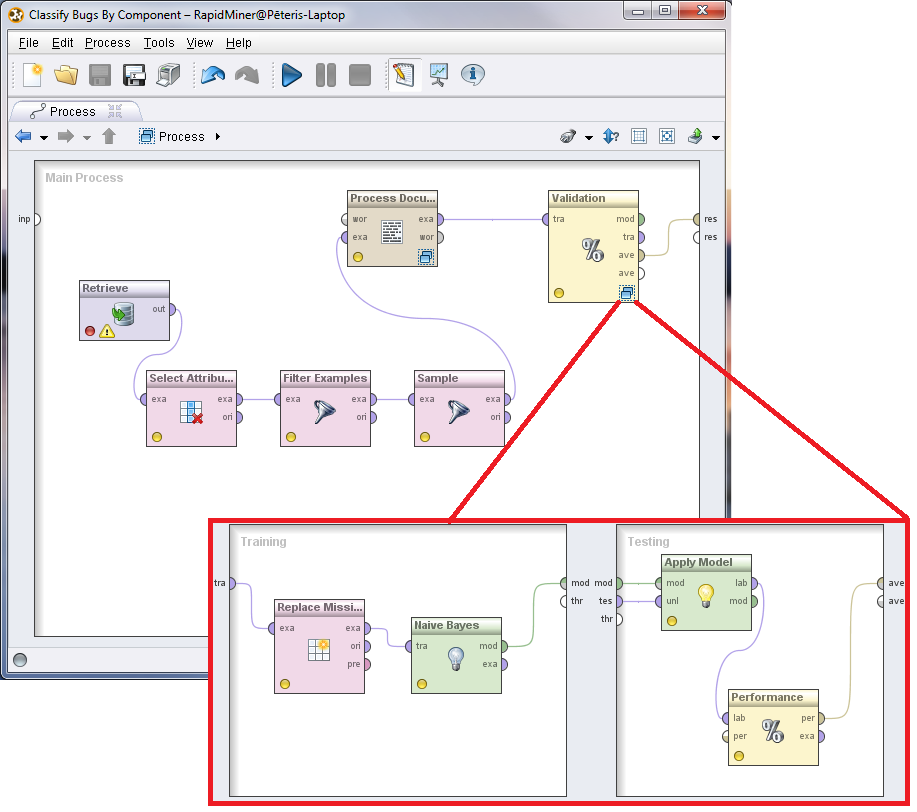
\includegraphics[scale=0.5]{ml3_classification_component_rapidminer}
\caption{Workflow in Rapid Miner: 1. Load data 2. Select attributes 3. Use only labeled data 4. Use a sample 5. Text processing 6. Cross Validation}
\end{center}
\end{figure}

Obtained results are displayed in the following table. Type is the class of algorithms, algorithm is a specific classification algorithm (Weka means that it wasn't a Rapid Miner implementation of the algorithm), sample is the number of classified bugs used, time is how long it took to run, accuracy is the stratified 10-fold cross validation result. Starred times indicate that they were run on a different computer.
\\
\\
\begin{tabular}{|c|c|c|c|c|}
\hline
Type     &       Algorithm    & Sample Size &  Time &  Accuracy   \\
\hline
\hline
Decision Trees & Weka J48      &   500  &   2:19  &    44.80\%  \\
                              &&  1000  &  10:25  &    45.50\%  \\
Decision Trees & Weka LAD-Tree &   500  &  13:40  &    39.80\%  \\

Bayes Classifiers & Naive Bayes &   500  &   0:08  &    37.80\%  \\
                               &&  1000  &   0:20  &    39.30\%  \\
                               &&  2000  &   0:56  &    42.40\%  \\
                               &&  4000  &   2:53  &    43.32\%  \\

Bayes Classifiers & Bayes Network &   500  &  0:18  &   40.60\%  \\
                                 &&  1000  &  1:11  &   42.50\%  \\
                                 &&  2000  &  4:06  &   50.05\%  \\
                                 &&  4000  & 43:41* &   54.45\%  \\

Lazy Classifiers & k-NN (k=1) &   500  &   0:09  &    41.60\%  \\
                             &&  1000  &   0:39  &    40.80\%  \\
                             &&  2000  &   3:08  &    46.65\%  \\
                             &&  4000  &  11:14* &    49.07\%  \\

Lazy Classifiers & k-NN (k=15) &   500  &   0:11  &    45.40\%  \\
                              &&  1000  &   0:38  &    49.80\%  \\
                              &&  2000  &   3:13  &    55.60\%  \\
                              &&  4000  &  11:18* &    58.02\%  \\

Lazy Classifiers & k-NN (k=30) &   500  &   0:10  &    45.00\%  \\
                              &&  1000  &   0:35  &    49.20\%  \\
                              &&  2000  &   3:01  &    54.60\%  \\
                              &&  4000  &  11:15* &    57.98\%  \\

Lazy Classifiers & k-NN (k=60) &   500  &   0:08  &    42.20\%  \\
                              &&  1000  &   0:38  &    46.70\%  \\
                              &&  2000  &   3:29  &    52.50\%  \\
                              &&  4000  &  11:21* &    56.10\%  \\

Support Vector Classifiers & Weka SMO &   500  &  0:53  &    41.40\%  \\
                                     &&  1000  &  4:15  &    47.20\%  \\
\hline
\end{tabular}
\\
\\

{\bf Conclusion.} As can be seen, it is possible to automatically classify bugs by their content more than half of the time. Most of the trialed algorithms could easily reach the 40\% accuracy barrier, however, the performance between these algorithms varies. While decision trees provide an acceptable although below average accuracy compared to all other algorithms, their performance is very poor. Bayes Network was the first algorithm to cross the 50\% line but it was beaten by k-NN which not only performs much faster but also gives the best accuracy. Therefore the k-NN algorithm was chosen to be run on the whole dataset to find out the best possible accuracy. It was mentioned in the lectures that the k-value should be in tens which clearly holds true in our experiments.

When the k-NN (k=15) was run on the whole dataset (4731 bugs), its accuracy was 58.55\%. If a more sophisticated tokenizer was developed and used, it's our belief that the accuracy could be higher, perhaps even as high as 70\%. Such accuracy is acceptable although leaves something to be desired and the model could be used to automatically assign the appropriate component when a bug is reported and the maintainers would only need to change it 40\% of the time.

% subsection Classification of bugs bugs by component (end)

% section Classification (end)

